\begin{figure}[h]
    \centering
    \definecolor{clrMental}{HTML}{4E79A7}
    \definecolor{clrTemporal}{HTML}{F28E2B}
    \definecolor{clrPerformance}{HTML}{59A14F}
    \definecolor{clrEffort}{HTML}{E15759}
    \definecolor{clrFrustration}{HTML}{B07AA1}
    \resizebox{\linewidth}{!}{%
    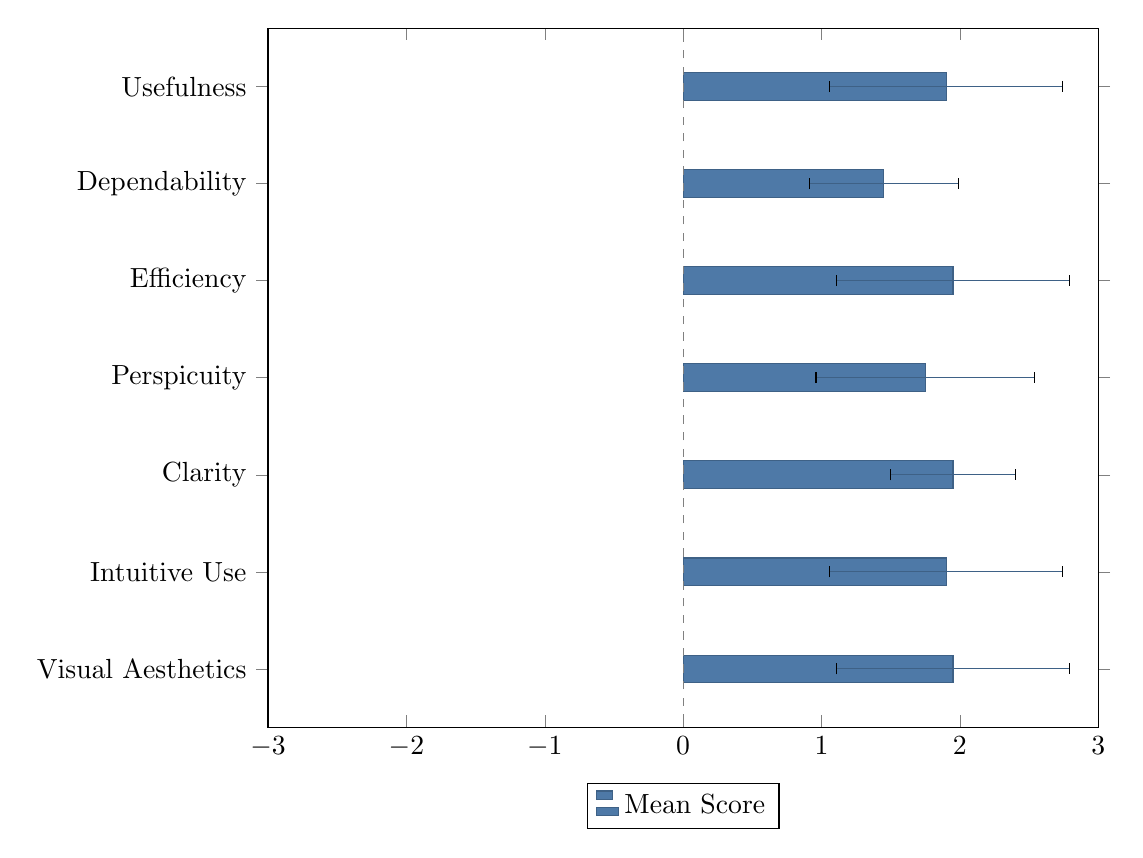
\begin{tikzpicture}
        \begin{axis}[
            xbar,
            ytick={1, 2, 3, 4, 5, 6, 7},
            yticklabels={Visual Aesthetics, Intuitive Use, Clarity, Perspicuity, Efficiency, Dependability, Usefulness},
            width=\linewidth,
            xmin=-3,
            xmax=3,
            xtick={-3,-2,-1,0,1,2,3},
            enlarge y limits=0.1,
            legend style={
                at={(0.5,-0.08)},
                anchor=north,
                legend columns=-1,
            },
        ]
        % y=1 Visual Aesthetics, y=2 Intuitive Use, y=3 clarity, y=4 Perspicuity,
        % y=5 Efficiency, y=6 Dependability, y=7 Usefulness
        % Scale importances
        %\addplot[
        %    fill=clrTemporal, draw=clrTemporal!80!black,
        %    error bars/.cd, x dir=both, x explicit,
        %] coordinates {
        %    (0.60,-3) +- (1.82,0)
        %    (1.80,-2) +- (0.45,0)
        %    (1.20,-1) +- (0.84,0)
        %    (2.40, 0) +- (0.55,0)
        %    (2.20, 1) +- (0.84,0)
        %    (1.60, 2) +- (1.14,0)
        %    (2.20, 3) +- (1.30,0)
        %};
        % Scale ratings
        \addplot[
            fill=clrMental, draw=clrMental!80!black,
            error bars/.cd, x dir=both, x explicit,
        ] coordinates {
            (1.95, 1) +- (0.84,0)
            (1.90, 2) +- (0.84,0)
            (1.95, 3) +- (0.45,0)
            (1.75, 4) +- (0.79,0)
            (1.95, 5) +- (0.84,0)
            (1.45, 6) +- (0.54,0)
            (1.90, 7) +- (0.84,0)
        };

        \draw[dashed, gray] (axis cs:0,-4) -- (axis cs:0,9);

        \legend{Mean Score}
        \end{axis}
    \end{tikzpicture}}%
    \caption{Mean scores of the UEQ+ sclaes}
    \label{fig:ueq-bar-graph-2}
\end{figure}